\begin{frame}{The standard model of particle physics}
\begin{columns}
\begin{column}{0.6\textwidth}
\begin{figure}
    \centering
    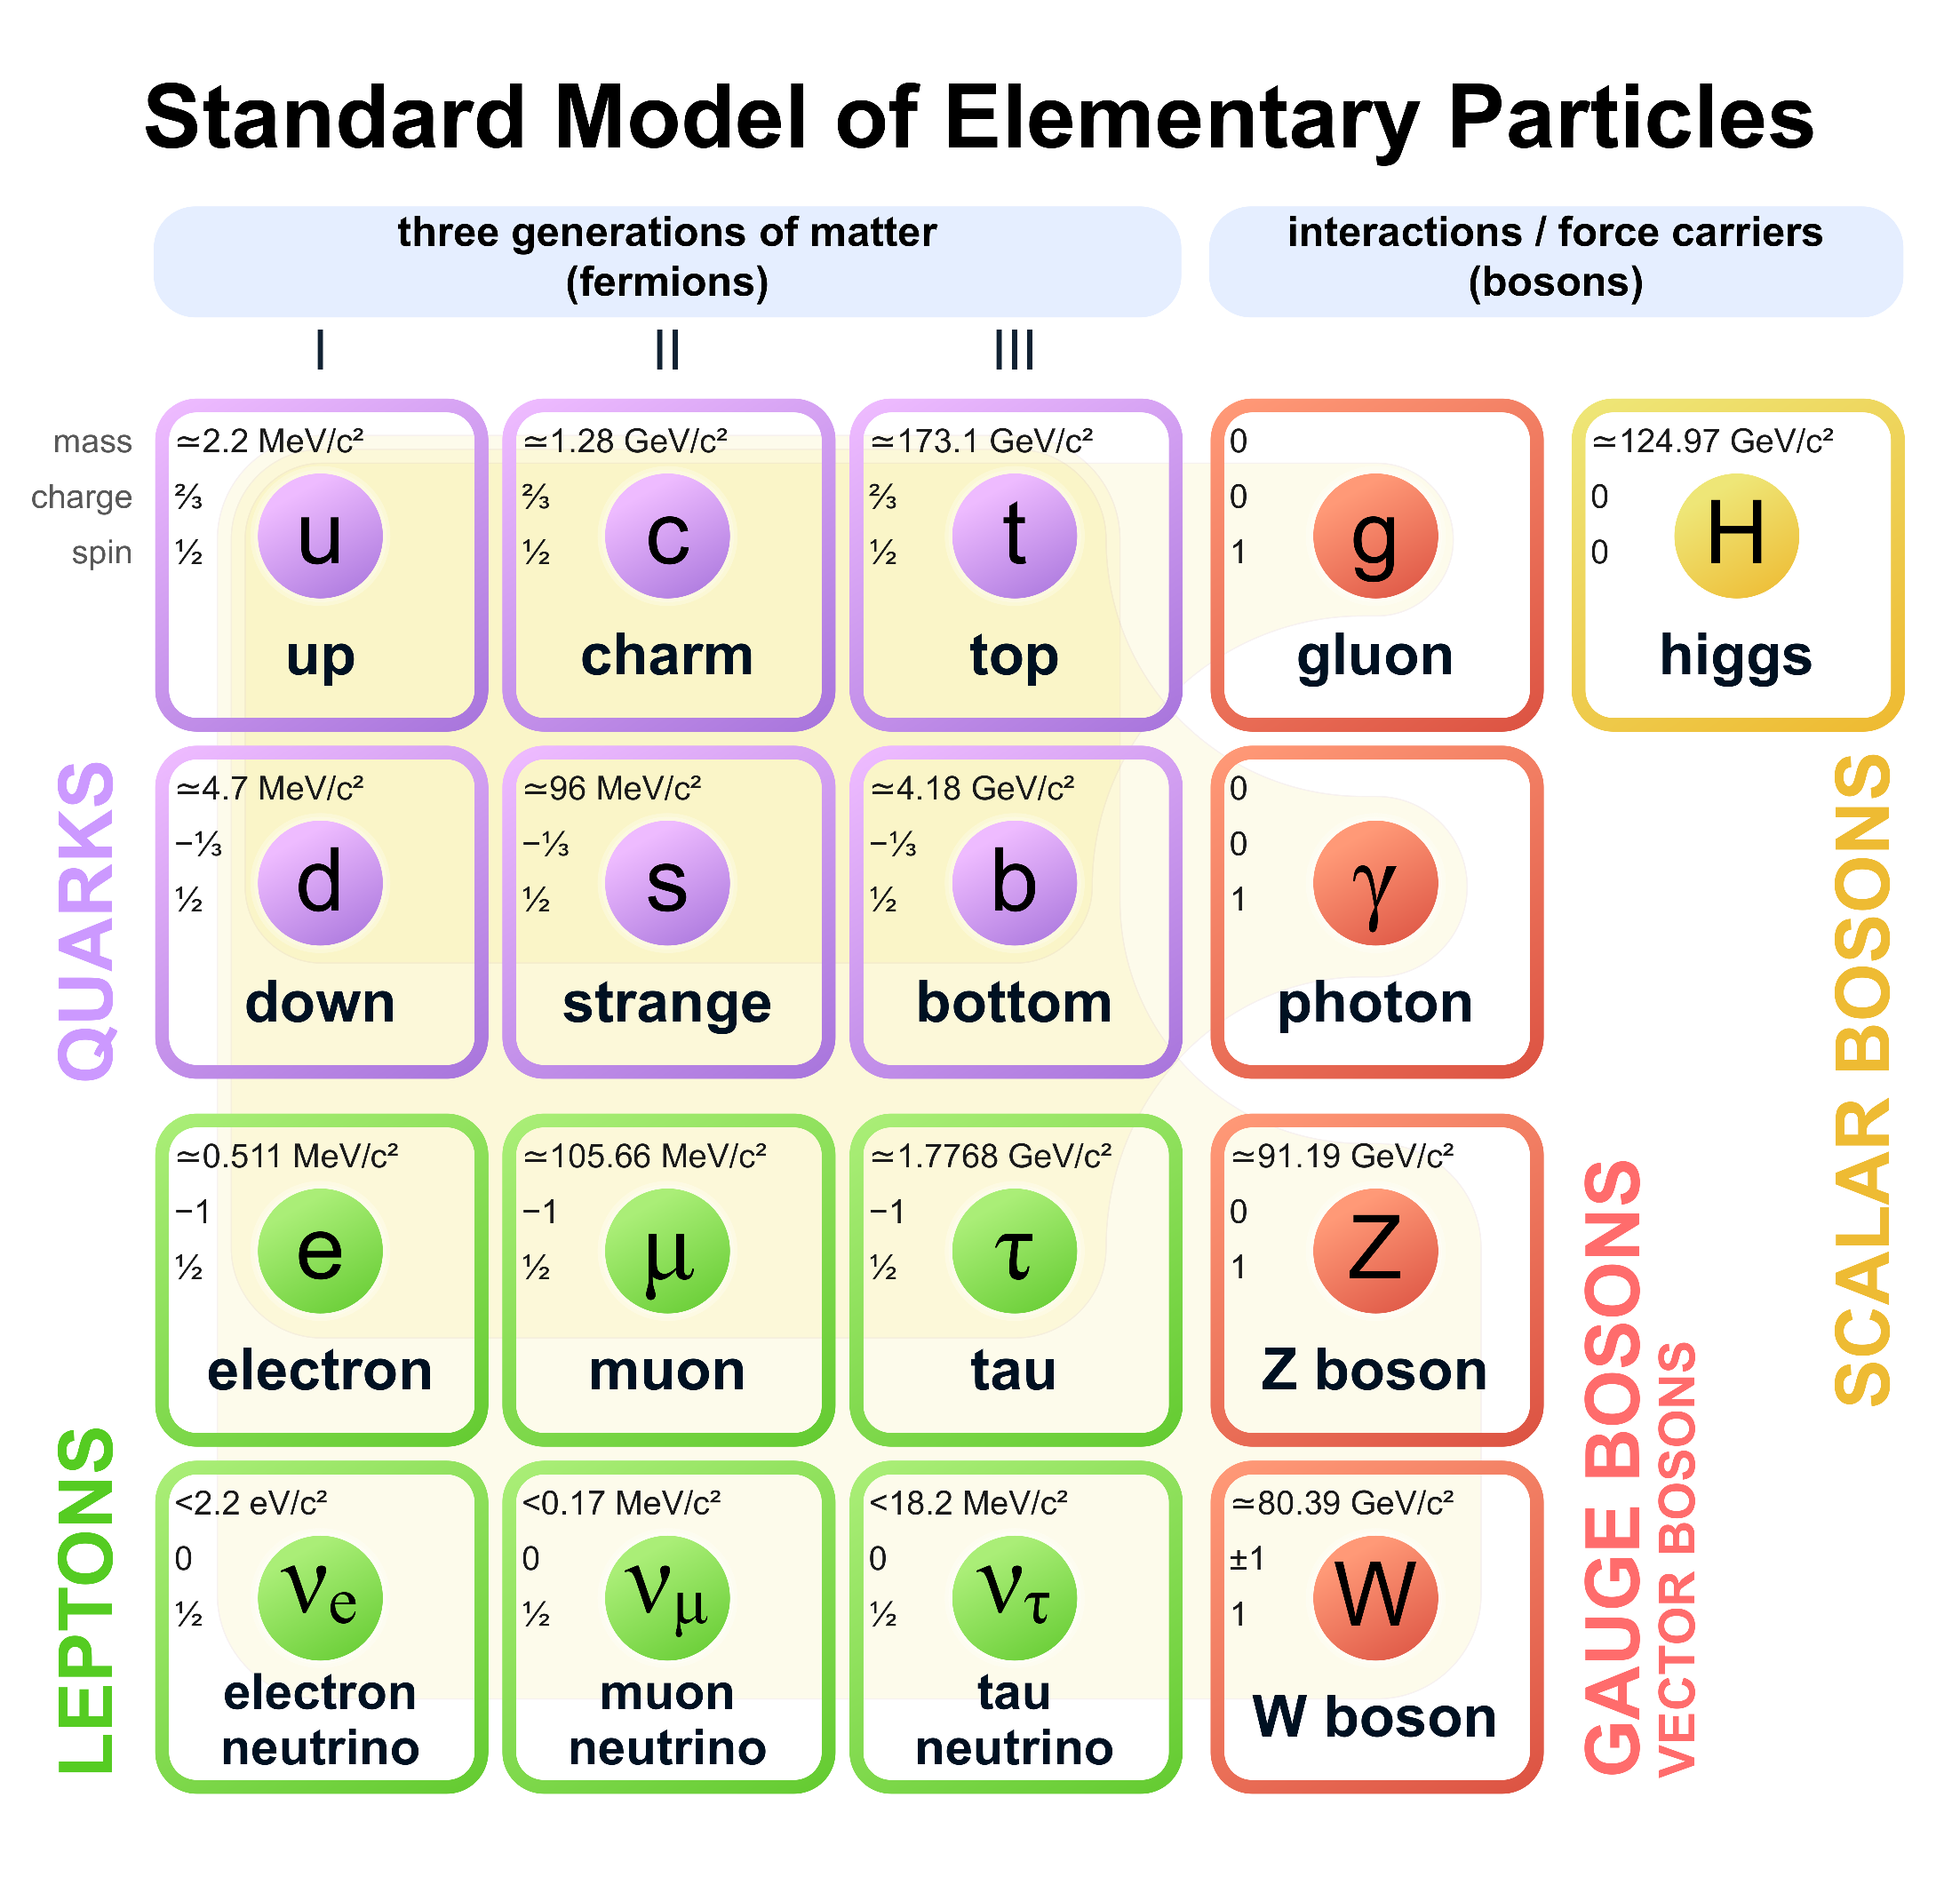
\includegraphics[scale=0.17]{Standard_Model_of_Elementary_Particles.eps}
\end{figure}
\end{column}
\pause
\begin{column}{0.4\textwidth}
\begin{block}{The top-quark}
        \begin{itemize}
            \item $ m \sim \SI{173}{\GeVovercsq}$
            \vspace{0.2cm}
            \item $\tau \sim \SI{5e-25}{\second}$
            \vspace{0.2cm}
            \item Lifetime < typical hadronisation time 
            \vspace{0.2cm}
            \item Decay into a \Pbottom-quark and a \PW-boson
        \end{itemize}
\end{block}
\end{column}
\end{columns}

\end{frame}

\begin{frame}{Top production}
    \begin{columns}
        \begin{column}{0.5\textwidth}
            \vspace{-0.4cm}
        \begin{block}{\tW single top production}
        \end{block}
			\begin{figure}
	            \centering
	            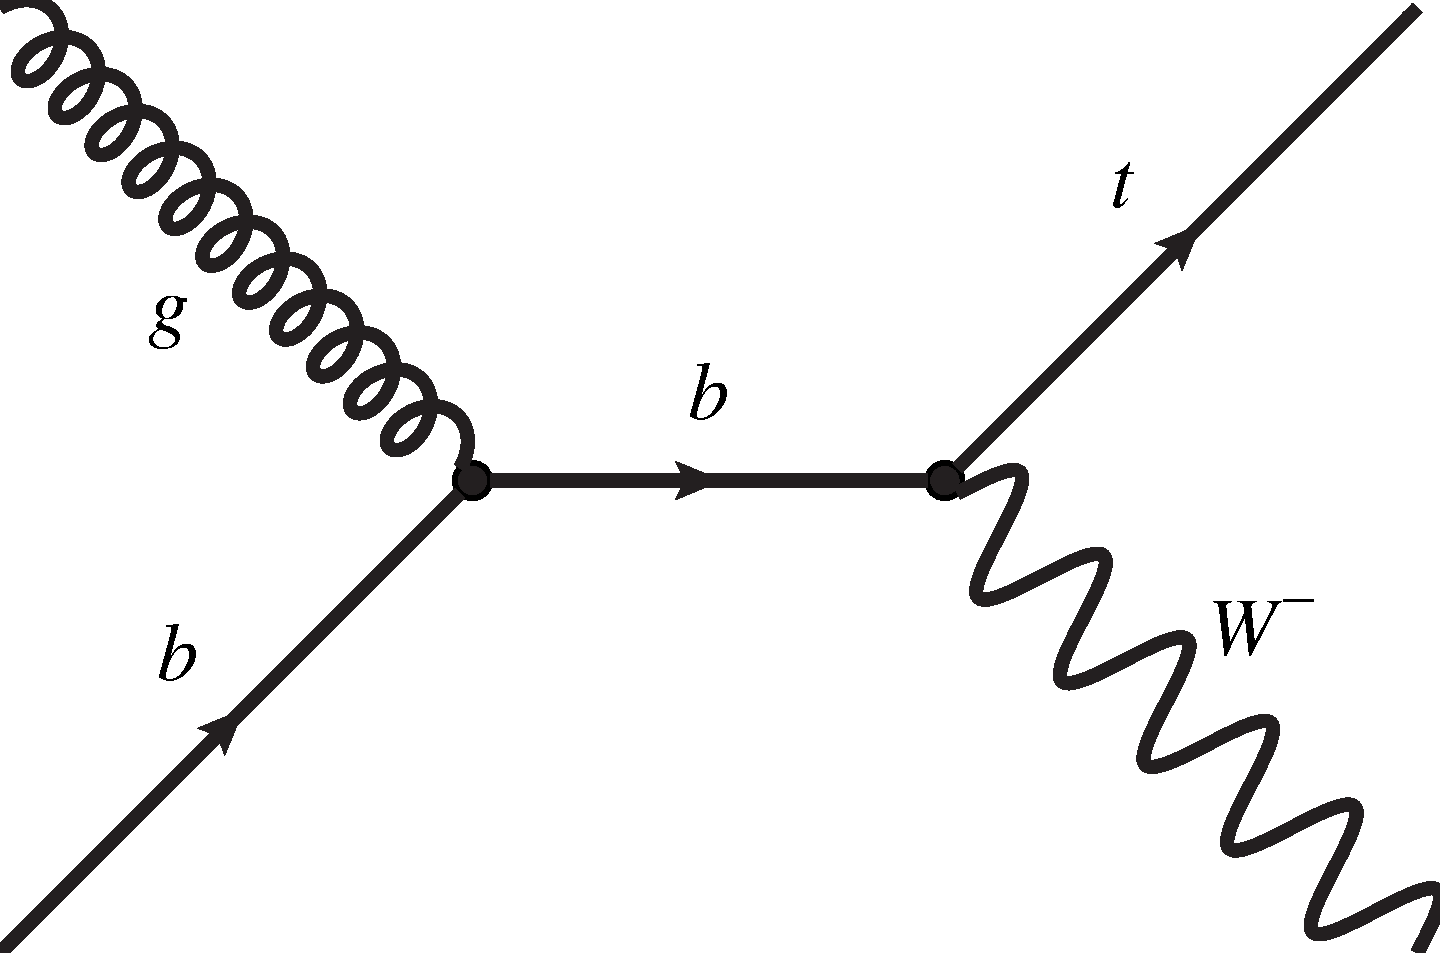
\includegraphics[width=0.8\textwidth]{tW_channel}
	        \end{figure}
	        \begin{itemize}
	        \item Via weak interaction
	        \item Relatively small cross section
	        \end{itemize}
        \end{column}
        \begin{column}{0.5\textwidth}
        \begin{block}{\ttbar pair production}
        \end{block}
        \begin{figure}
            \centering
            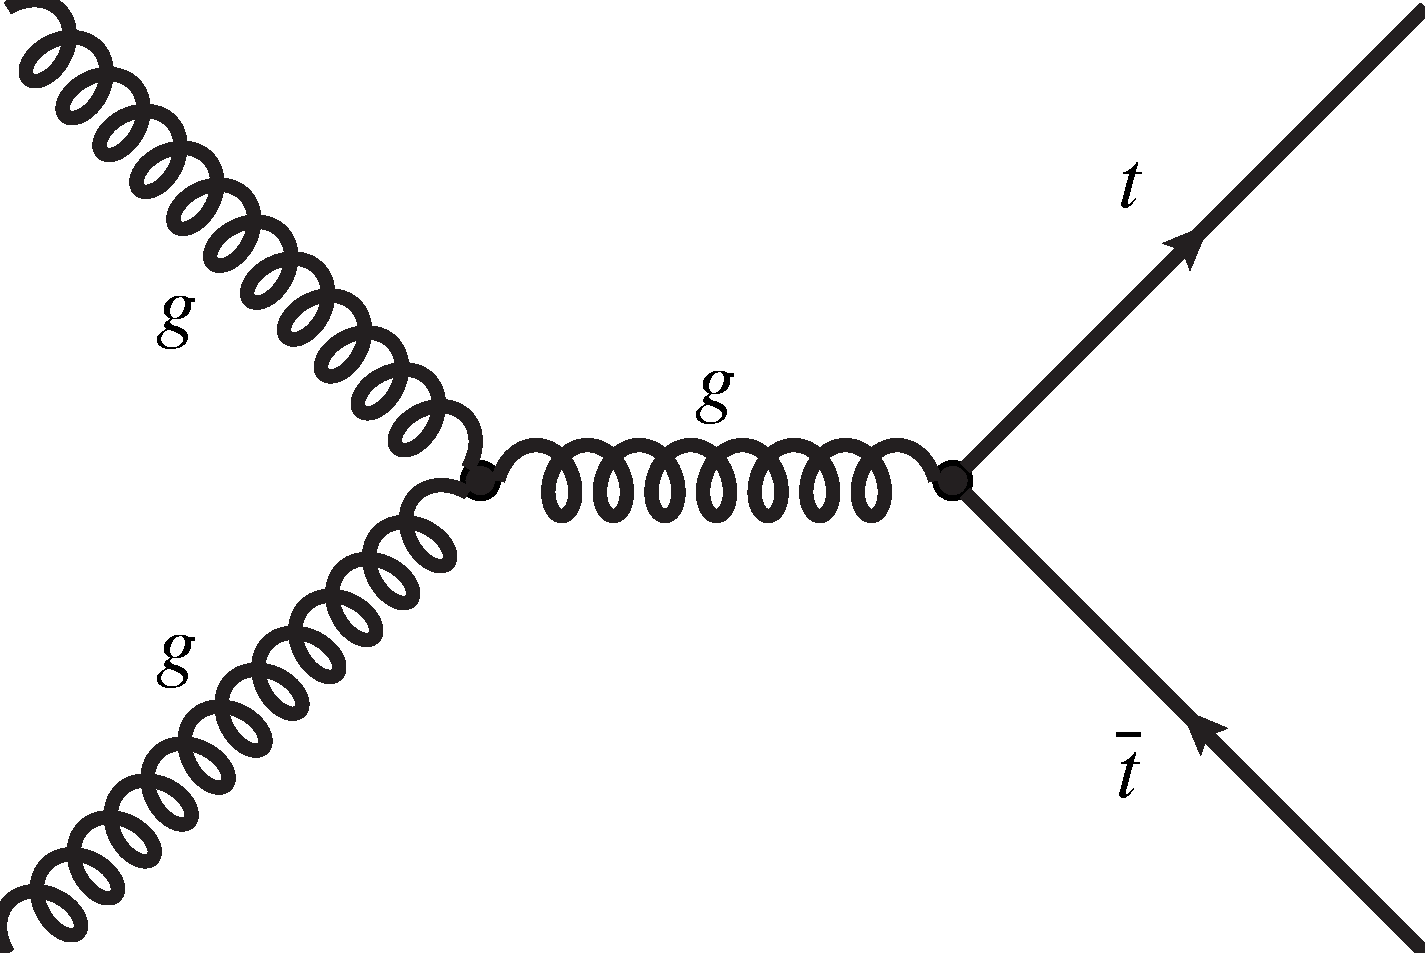
\includegraphics[width=0.8\textwidth]{ttbar_ttbar_1-BW}
        \end{figure}
        \begin{itemize}
        	\item Via strong interaction
        	\item Over 10 times larger cross-section
        \end{itemize}
        \end{column}
    \end{columns}
\end{frame}

\begin{frame}{The Large Hadron Collider - LHC}
\begin{columns}
\begin{column}{0.7\textwidth}
\begin{figure}
        \centering
        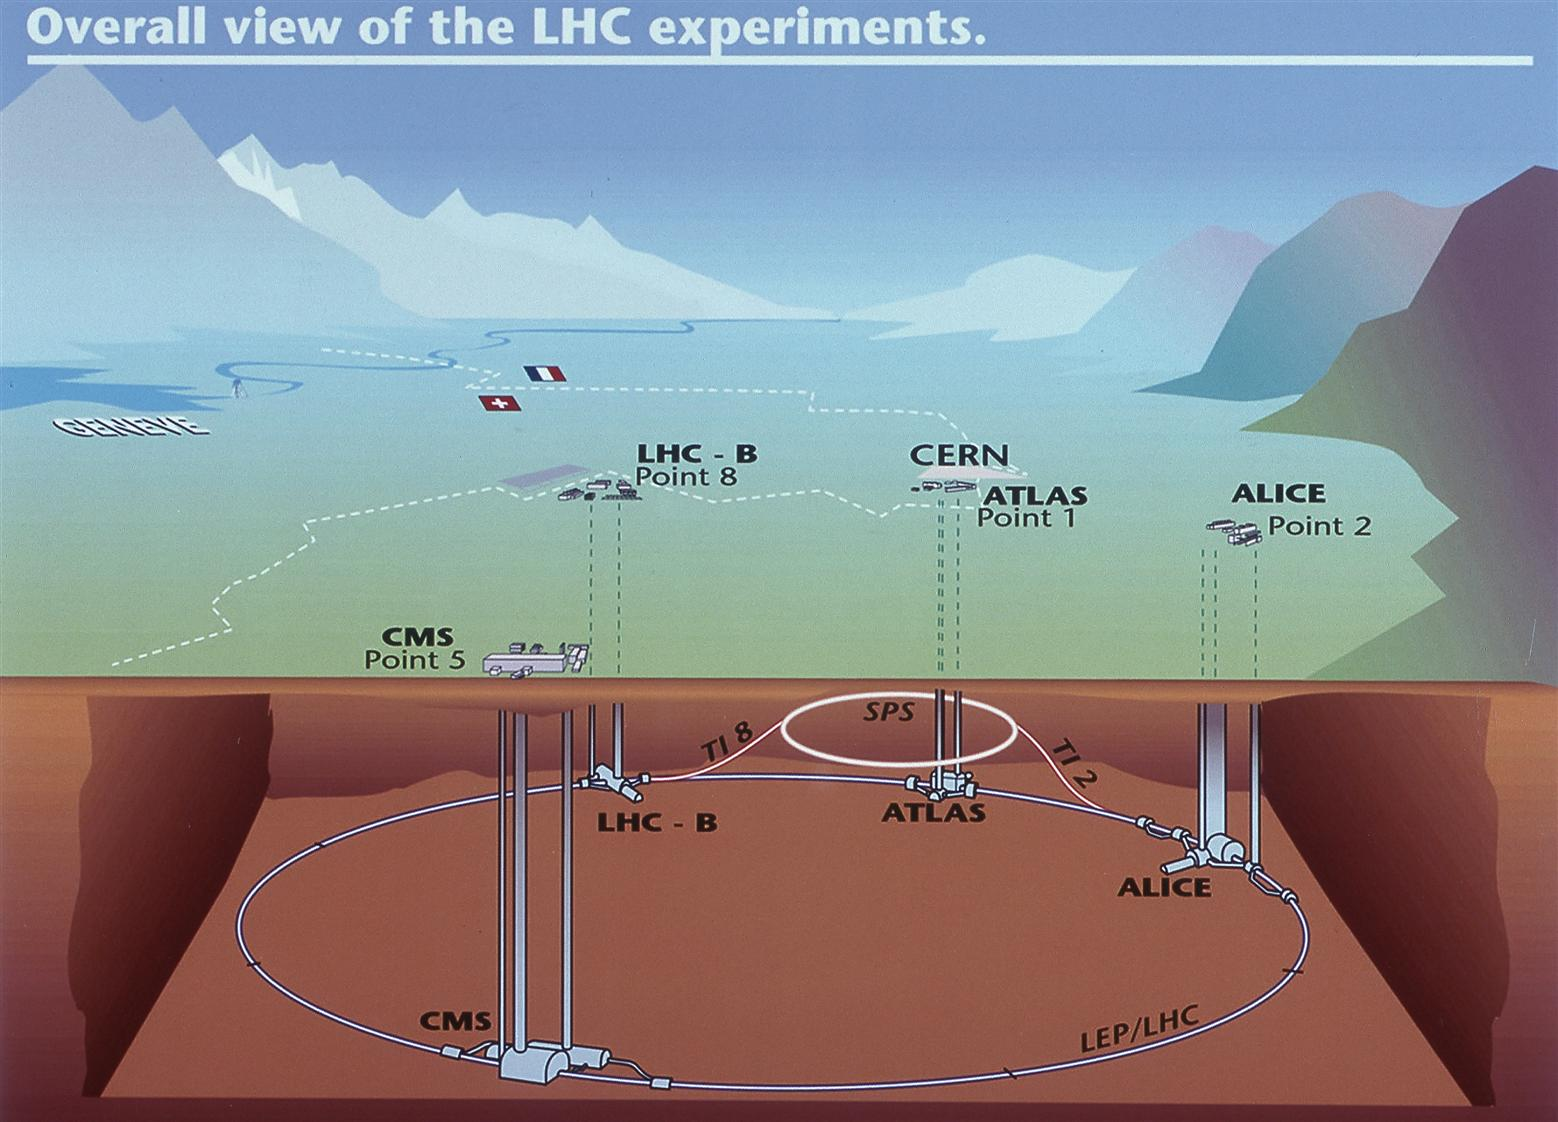
\includegraphics[width=0.9\textwidth]{CERN-all-experiments}
        %\caption{\cite{Pequenao:1095924}}
\end{figure}
\end{column}
\begin{column}{0.5\textwidth}
\begin{itemize}
\item Proton-proton collider
\vspace{0.3cm}
\item $\mysim$ \SI{27}{\kilo \metre} circumfence
\vspace{0.3cm}
\end{itemize}
	     \begin{align*}
	        \hfsetfillcolor{logo_blue!10}
	        \hfsetbordercolor{logo_blue}
	        \tikzmarkin{a1}(0.3,-0.3)(-0.3,0.55)
	        E_{CM} &= \SI{13}{\tera \electronvolt}\\ 
	        \mathcal{L} &= \SI{1.5e34}{\per \square \centi \metre  \per \second} 
	        \tikzmarkend{a1}
	    \end{align*}
\end{column}
\end{columns}
\end{frame}

\begin{frame}{The ATLAS experiment}
    \begin{figure}
        \centering
        \includegraphics[width=0.8\textwidth]{lhc_atlas_combination.eps}
        %\caption{\cite{Pequenao:1095924}}
        \label{fig:my_label}
    \end{figure}
\end{frame}

\begin{frame}{ATLAS - a genereal purpose detector}
    \begin{figure}
        \centering
        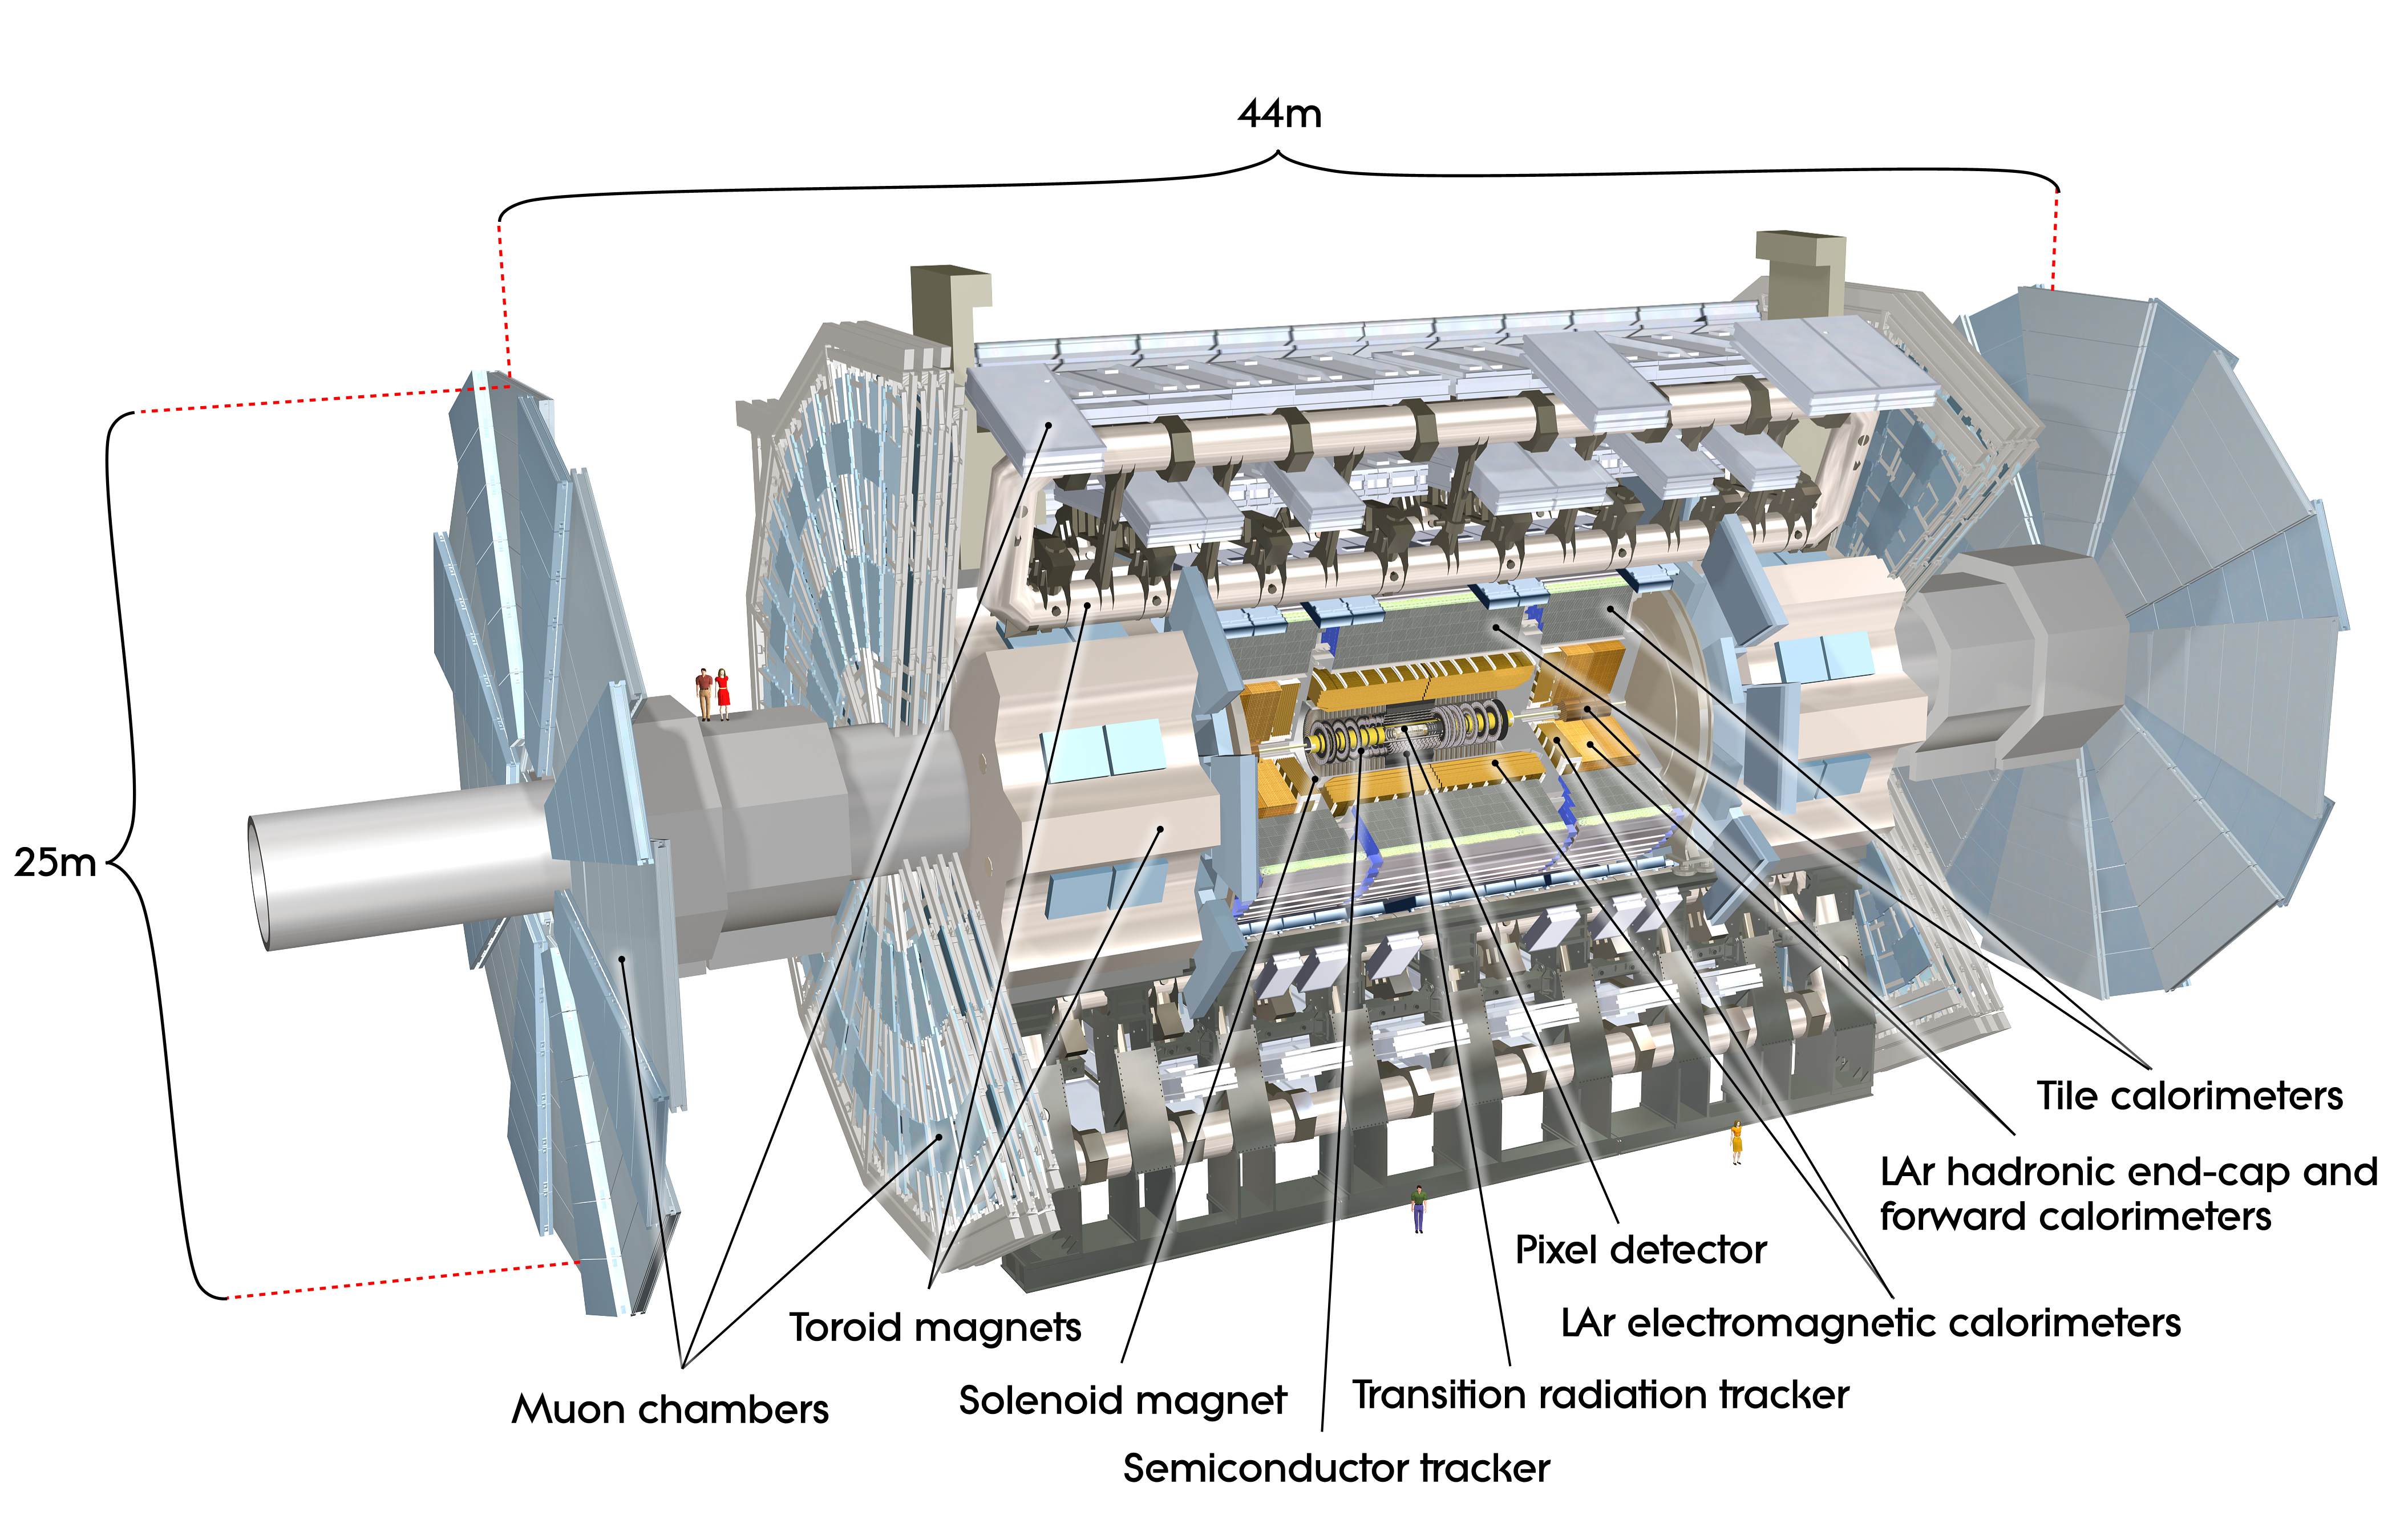
\includegraphics[width=0.8\textwidth]{atlas_detector.jpg}
        %\caption{\cite{Pequenao:1095924}}
        \label{fig:my_label}
    \end{figure}
\end{frame}


\begin{frame}{ATLAS - object identification}
    \begin{figure}
        \centering
        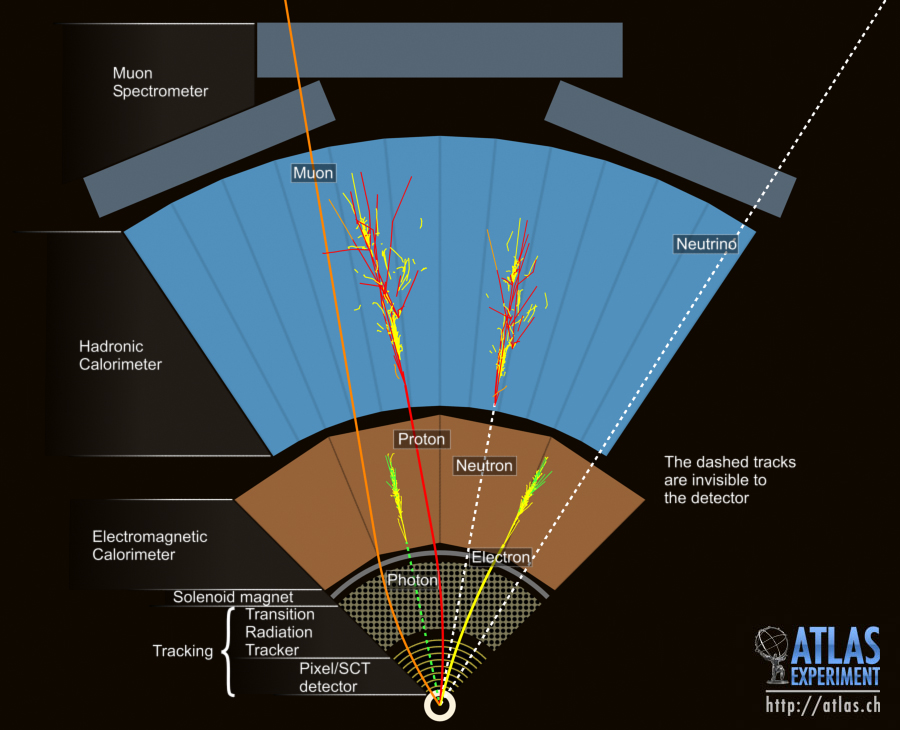
\includegraphics[width=0.8\textwidth]{figures_theory/atlas_quer.jpg}
        %\caption{\cite{Pequenao:1095924}}
        \label{fig:my_label}
    \end{figure}
\end{frame}



\begin{frame}{\tW to \ttbar separation at LO}
\begin{columns}
\quad
    \begin{column}{0.45\textwidth}
    \begin{block}{\tW decay}
    \end{block}
    \end{column}
    \quad
    \begin{column}{0.45\textwidth}
    \begin{block}{\ttbar decay}
    \end{block}
    \end{column}
\quad
\end{columns}
    \begin{figure}[htbp]
    \centering
    \begin{subfigure}[b]{0.4\textwidth}
        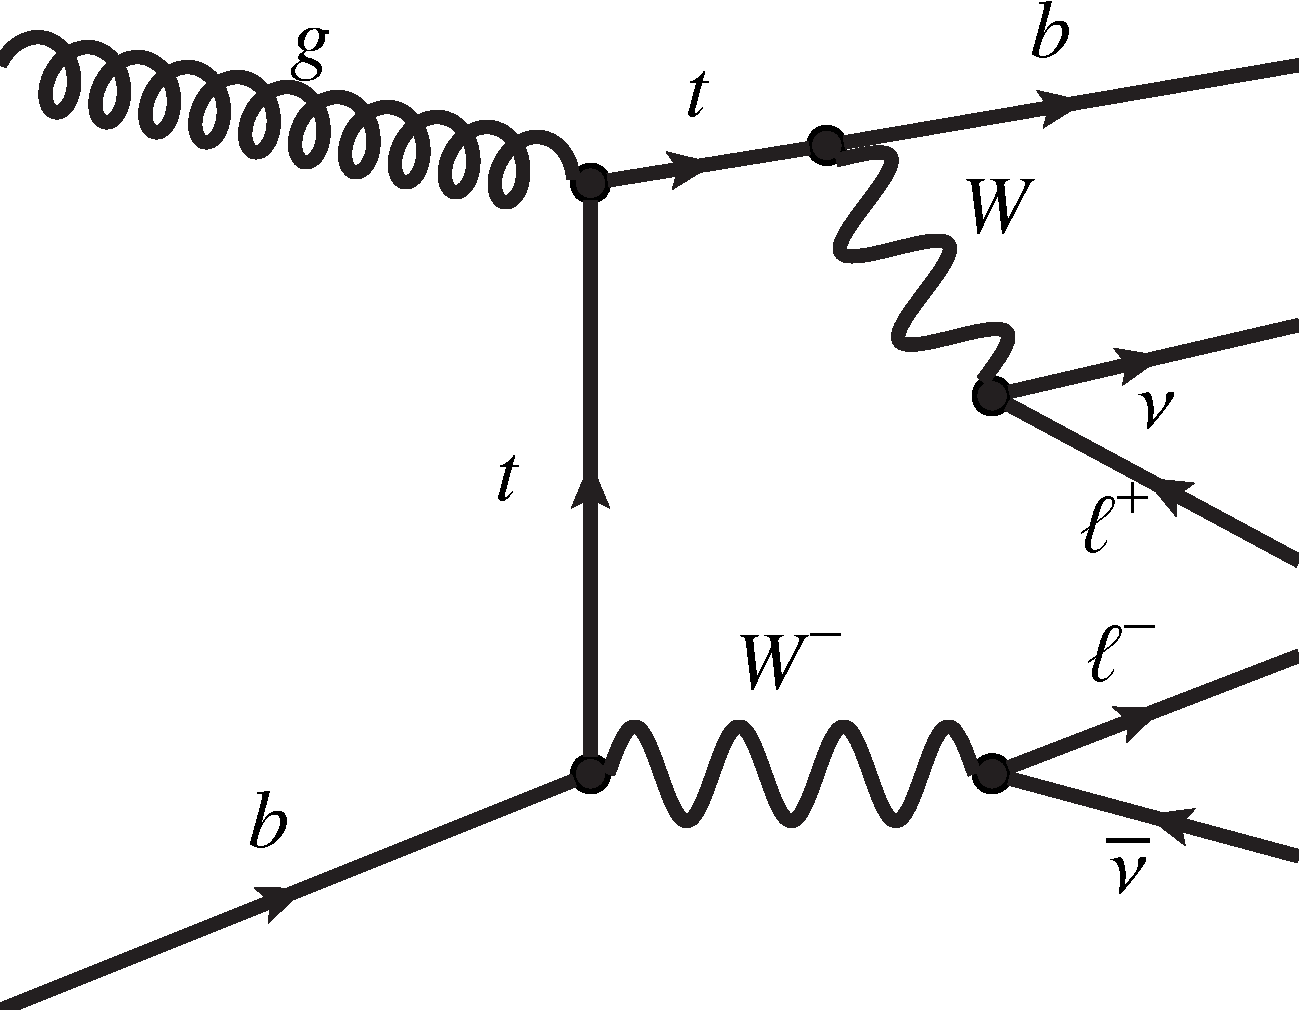
\includegraphics[width=\textwidth]{feynman_diagrams/tW-decay.pdf}
        \label{fig:nlo:tw}
    \end{subfigure}
\quad
    \begin{subfigure}[b]{0.4\textwidth}
        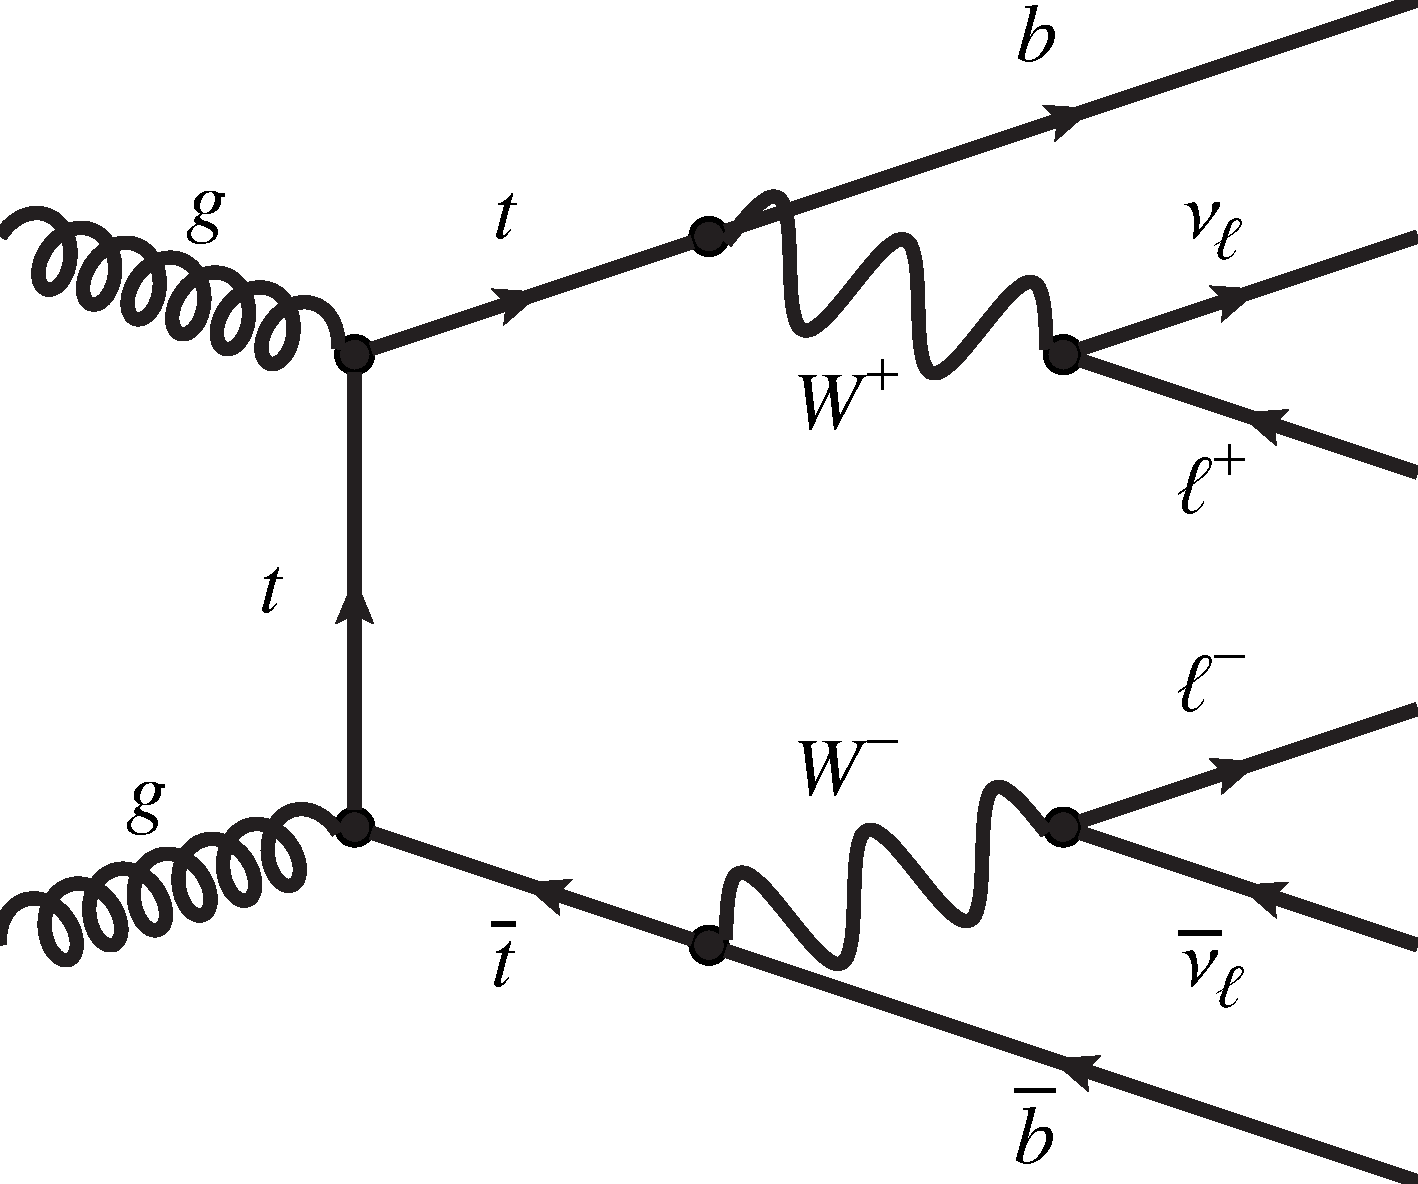
\includegraphics[width=\textwidth]{ttbar-decay}
        \label{fig:nlo:ttbar}
    \end{subfigure}
\end{figure}
\begin{columns}
\quad
    \begin{column}{0.45\textwidth}
	\begin{itemize}
	\item $\sigma_{\tW} \sim \SI{71.7}{\pico\barn}$
	\item 2 \PW, 1 \Pbottom
	\end{itemize}
    \end{column}
    \quad
    \begin{column}{0.45\textwidth}
	\begin{itemize}
	\item $\sigma_{\ttbar} \sim \SI{832}{\pico\barn}$
	\item Final state: 2 \PW, 2 \Pbottom
	\end{itemize}
    \end{column}
\quad
\end{columns}
\end{frame}

